% \section{Resolving the Insufficiency with an Ontology}

% If a family name is the most common form of partial evidence, an ontology
% should be able to use it. We decompose this into three steps: identify the
% family from the page, list its members, and choose among them.

% \subsection{Design}

% We use the 410 indication and contraindication edges whose text names only
% the family, in Wikipedia and PubMed together. A pick counts as correct when it
% is any disease the drug has the same relation to, since a family list holds
% 2.47 true answers on average and over half hold more than one.

% \paragraph{Listing the members.}
% The \emph{given-family} list takes the narrowest ancestor of the answer that
% the text names and lists its MONDO descendants up to two levels below it,
% capped at 64. It assumes the right family is known. The \emph{page-built} list
% instead finds every MONDO category with at least two children whose name
% appears in the drug's Wikipedia article, and takes the union of their
% descendants. A list larger than 64 candidates counts as too broad.

% \paragraph{Choosing a member.}
% We compare Qwen2.5-7B choosing from the given-family list without the page
% and with it; Wikipedia evidence (the candidate's own article names the drug);
% PubMed evidence (the number of abstracts naming both the drug and the
% candidate, with a relation-specific qualifier); PubMed evidence normalized by
% the candidate's total number of abstracts; and a popularity prior, the
% candidate with the most PubMed abstracts regardless of the drug. Two baselines
% use no ontology: a list of the same size with the answer and random diseases,
% and the same list with the page in the prompt, which is what a standard RAG
% system sees. Paired comparisons use McNemar's test \citep{mcnemar1947}.

% \subsection{Results}

% \begin{figure}[t]
% \centering
% \includegraphics[width=\columnwidth]{fig_recovery.pdf}
% \caption{Recovery on 410 family-only facts. Blue and gray bars choose within
% the given family; hatched bars do not receive the family.}
% \label{fig:recovery}
% \end{figure}

% \begin{table}[t]
% \centering
% \small
% \setlength{\tabcolsep}{4pt}
% \begin{tabular}{lcc}
% \toprule
%  & Given family & Page-built \\
% \midrule
% Usable lists (of 410) & 410 & 166 \\
% List contains the sampled answer & 98.5\% & 19.8\% \\
% List contains any true answer & 99.5\% & 24.6\% \\
% Median list size & 14 & 32 \\
% \bottomrule
% \end{tabular}
% \caption{Candidate lists. Coverage is over all 410 facts; of the 244 unusable
% page-built lists, 209 exceed 64 candidates and 35 have no usable category.}
% \label{tab:lists}
% \end{table}

% \paragraph{Given the family, the ontology narrows the search well.}
% Table~\ref{tab:lists} shows that when the right family is known, its member
% list contains the answer 98.5\% of the time with a median of 14 candidates.
% List coverage is not accuracy, however: a member still has to be chosen.

% \paragraph{Finding the family is the bottleneck.}
% When the list is built from the categories the page actually names, it
% contains the answer for only 19.8\% of facts. A page names a median of five
% categories, and for 209 of 410 facts their union exceeds 64 candidates. The
% page does name the right family, but it also names others, and nothing in the
% text marks which one belongs to the answer. Reading more text makes this worse,
% not better. Building the list from the Wikipedia article and the PubMed
% abstracts together raises the median number of categories named to 17; 391 of
% 410 lists then exceed 64 candidates, and only 3.7\% of facts get a usable list
% that contains the answer. The bottleneck is not missing text but too many
% candidate families.

% \paragraph{Within a family, popularity beats evidence.}
% Figure~\ref{fig:recovery} compares ways of choosing. Given the family, the
% model alone is right 35.9\% of the time, and 32.4\% when it also sees the
% page. PubMed co-mention also reaches 35.9\%, and taking evidence first
% (Wikipedia and PubMed combined) and the model's pick otherwise reaches 41.7\%,
% which beats the model alone (59 against 35 discordant facts, $p = 0.018$). The
% popularity prior, which ignores the drug, reaches 46.8\%, the highest of all.
% Once co-mention counts are divided by the candidate's total abstracts, they
% fall to 25.4\%, so the drug-specific part of the literature signal is weak.
% Wikipedia rarely helps, because a candidate's article names the drug in only
% 3.9\% of cases. The two baselines without an ontology reach 34.9\% (random
% list) and 32.7\% (page in prompt). Their lists exclude the drug's other true
% partners, so under any-true-answer scoring they are not at matched chance with
% the family lists and serve as reference points only.


% \paragraph{What the misses look like.}
% Some misses choose a better-studied member of the family (for carboplatin,
% ovarian carcinoma rather than the rarer germ cell tumor the graph records), and
% some are true facts the graph does not list (moxifloxacin for Legionnaires'
% disease), so evaluation against a graph understates recovery for every method
% alike. The supplement lists examples.

% \paragraph{End to end.}
% Without being given the family, building the list from the page and choosing
% by evidence recovers the answer for 10.0\% of facts. The page-in-prompt
% baseline reaches 32.7\%, helped by a family name that lets it eliminate
% random distractors outside the family. With lists built from both corpora,
% end-to-end recovery falls to 1.5\%, for the reason given above.



\section{Results and Analysis}

\subsection{Coarse evidence weakens abstention (\clade{})}

\begin{table}[t]
\centering
\small
\setlength{\tabcolsep}{2.9pt}
\begin{tabular}{llcccc}
\toprule
Model & Passage Type & Correct & Wrong & Declines & Prec. \\
\midrule
\multirow{3}{*}{Qwen2.5 7B} & named & 71.7 & 3.8 & 24.5 & 95.0 \\
 & family-only & 26.5 & 18.1 & 55.3 & 59.4 \\
 & silent & 13.8 & 2.5 & 83.8 & 84.6 \\
\midrule
\multirow{3}{*}{OLMo 2 7B} & named & 77.4 & 15.1 & 7.5 & 83.7 \\
 & family-only & 37.2 & 44.7 & 18.1 & 45.5 \\
 & silent & 30.6 & 24.4 & 45.0 & 55.7 \\
\midrule
\multirow{3}{*}{Granite 3.1 8B} & named & 72.6 & 7.5 & 19.8 & 90.6 \\
 & family-only & 30.2 & 26.5 & 43.3 & 53.3 \\
 & silent & 15.0 & 10.0 & 75.0 & 60.0 \\
\midrule
\multirow{3}{*}{Qwen2.5 0.5B} & named & 77.4 & 14.2 & 8.5 & 84.5 \\
 & family-only & 34.4 & 55.8 & 9.8 & 38.1 \\
 & silent & 28.7 & 50.6 & 20.6 & 36.2 \\
\midrule
\multirow{3}{*}{Qwen2.5 14B} & named & 67.9 & 2.8 & 29.2 & 96.0 \\
 & family-only & 24.2 & 17.2 & 58.6 & 58.4 \\
 & silent & 11.9 & 2.5 & 85.6 & 82.6 \\
\bottomrule
\end{tabular}
\caption{Open-book outcomes (\%) on PrimeKG questions where all four distractors come from the answer's MONDO neighborhood (106 named, 215 family-only, and 160 silent questions). Precision is the percentage of correct answers among questions where the model did not abstain.}
\label{tab:outcomes}
\end{table}

\begin{figure*}[t]
\centering
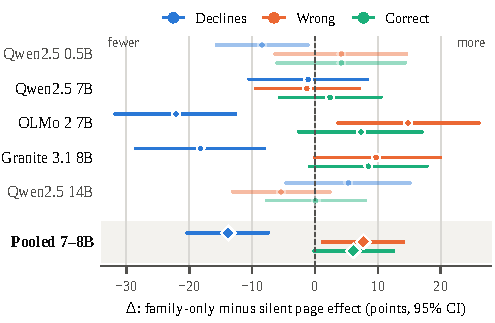
\includegraphics[width=\textwidth]{figures/fig_forest.pdf}
\caption{Isolating the effect of a coarse (\emph{family-only}) passage relative to an uninformative (\emph{silent}) passage. For each question, the page effect is the open-book outcome minus the closed-book outcome. Points show the mean page effect on family-only questions minus that on silent questions, with 95\% bootstrap confidence intervals. The pooled row averages page effects across the three 7--8B models (481 neighborhood-matched questions). Gray rows indicate models outside the 7--8B pooled set.}
\label{fig:forest}
\end{figure*}

\paragraph{Models abstain far less on family-only passages than on silent passages.}
Table~\ref{tab:outcomes} reports open-book performance when models read the retrieved passage. Across all three 7--8B models, seeing a coarse, family-only passage causes models to abstain much less often than seeing a silent passage: abstention drops from 83.8\% to 55.3\% on Qwen2.5-7B, from 45.0\% to 18.1\% on OLMo~2 7B, and from 75.0\% to 43.3\% on Granite~3.1 8B. Because the models attempt to answer many more questions without having the fine-grained facts, precision among answered questions drops sharply—ranging from 45.5\% to 59.4\% on family-only passages, compared to 83.7\% to 95.0\% on named passages.

\paragraph{Within-question controls confirm the effect comes from the passage.}
A raw comparison between passage groups partially reflects baseline differences between the facts in each group. Even without a passage (closed book), family-only questions yield more incorrect guesses than silent questions across all three 7--8B models (32.6\% versus 15.6\% on Qwen2.5-7B, 56.7\% versus 51.2\% on OLMo~2, and 33.0\% versus 26.2\% on Granite; see the supplement). Figure~\ref{fig:forest} removes this baseline gap by comparing each question against its own closed-book performance.

Pooled across the three 7--8B models, adding a silent passage increases abstention by 28.5 percentage points over closed-book answering, whereas adding a family-only passage increases abstention by only 14.7 points. This yields a net abstention reduction of $-13.8$ points on family-only passages relative to silent passages (95\% CI $-20.3$ to $-7.5$, $p = 3.6\times10^{-5}$, and $p = 1.1\times10^{-4}$ after Bonferroni correction across the three outcomes). The extra answers triggered by the family-only passage split roughly evenly between right and wrong guesses: relative to a silent passage, a family-only passage increases wrong answers by $+7.7$ points (95\% CI $1.2$ to $14.0$, $p = 0.019$) and increases correct answers by $+6.1$ points (95\% CI $-0.1$ to $12.4$, $p = 0.058$).

Examining models individually, the net drop in abstention is large and statistically significant for OLMo~2 ($-22.1$ points, $p = 6\times10^{-6}$) and Granite ($-18.2$ points, $p = 0.0006$), as well as Qwen2.5 0.5B ($-8.4$ points, 95\% CI $-15.7$ to $-1.1$, $p = 0.027$). Qwen2.5-7B shows a small differential page effect ($-1.1$ points, $p = 0.82$) because it already abstains less often on family-only questions closed book (32.1\% versus 59.4\%), and adding a passage increases its abstention rate by similar amounts in both groups.

\paragraph{Smaller disease families trigger stronger over-answering.}
The tendency to guess from a coarse passage depends on how specific the mentioned family is. When we divide family-only questions into thirds based on the number of diseases in the mentioned MONDO family, the pooled abstention drop is strong for small families with $\le 10$ members ($-17.3$ points, 95\% CI $-26.2$ to $-8.2$) and medium families with 11--20 members ($-18.4$ points, 95\% CI $-26.6$ to $-10.3$), but weakens to $-6.5$ points (95\% CI $-15.7$ to $+3.0$) for large families with more than 20 members (Figure~\ref{fig:fixes}c). Narrower categories make an insufficient passage appear even more answerable.

\subsection{Counterfactual Edits Prove the Family Name Causes \clade{}}

\begin{figure}[t]
\centering
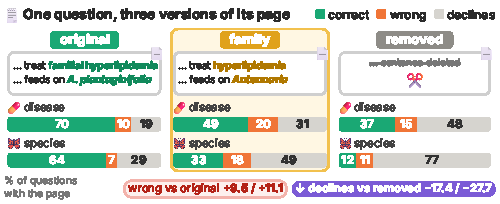
\includegraphics[width=\columnwidth]{figures/fig_example.pdf}
\caption{Counterfactual edits on identical questions for biomedical facts (PrimeKG, 130 questions) and ecological interactions (GloBI, 255 questions). The \emph{family} edit replaces every mention of the exact answer with its parent category; the \emph{removed} edit deletes sentences mentioning the answer. Bars show open-book outcomes (\%) averaged across the three 7--8B models.}
\label{fig:edit}
\end{figure}

Figure~\ref{fig:edit} shows the results of our counterfactual experiment, where the exact same 130 questions are evaluated with three versions of the same passage (\emph{original} named, \emph{family} replacement, and sentence \emph{removed}).

Compared to the original passage that names the exact disease, replacing the disease name with its parent family lowers correct answers by 21.0 percentage points (95\% CI $-26.9$ to $-15.6$) and increases wrong answers by 9.5 points (95\% CI $5.9$ to $13.6$), while abstention rises by only 11.5 points (95\% CI $7.4$ to $15.9$). More importantly, compared to deleting the answer sentence entirely (\emph{removed}), leaving the coarse family name in the passage reduces abstention by 17.4 points (95\% CI $-23.6$ to $-11.5$), while increasing wrong answers by 5.1 points (95\% CI $0.5$ to $10.3$) and correct answers by 12.3 points (95\% CI $6.9$ to $17.9$). Every individual model follows this exact ordering: from the \emph{removed} passage to the \emph{family} passage, abstention drops from 70.0\% to 43.8\% on Qwen2.5-7B, from 56.2\% to 40.8\% on Granite, and from 18.5\% to 7.7\% on OLMo~2. Thus, the presence of a coarse category name directly suppresses abstention and induces unreliable guessing.

\subsection{Why Simple Mitigation Strategies Fail}

\begin{figure*}[t]
\centering
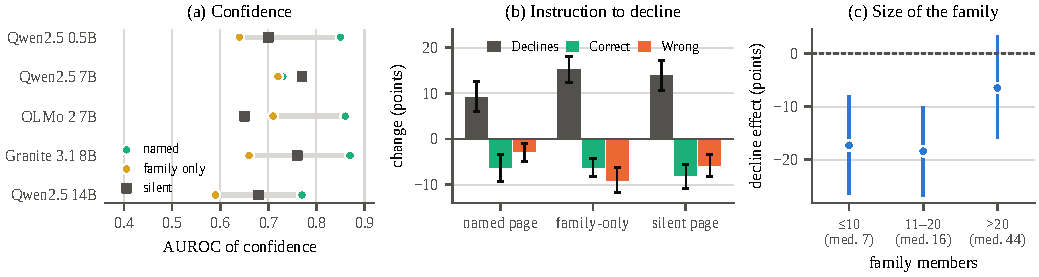
\includegraphics[width=\textwidth]{figures/fig_fixes.pdf}
\caption{Evaluating three candidate fixes for \clade{}. (a) Answer confidence separates correct from wrong answers poorly on family-only passages across all models. (b) An explicit prompt instruction to abstain on broad categories increases abstention indiscriminately across all passage types, including named passages that contain the exact answer (pooled 7--8B models, 95\% CIs). (c) The abstention drop caused by family-only passages is strongest when the mentioned family has 20 or fewer members.}
\label{fig:fixes}
\end{figure*}

\paragraph{Model confidence fails to flag coarse-evidence guesses.}
A natural defense is to abstain whenever the model's answer probability falls below a threshold. However, Figure~\ref{fig:fixes}a shows that answer confidence is much worse at separating right from wrong answers on family-only passages (AUROC 0.59--0.72) than on named passages (AUROC 0.73--0.87) across every model tested. When models guess wrong on a family-only passage, they do so with high confidence: the mean probability assigned to incorrect answers is 0.77--0.99 across the 7B--14B models, reaching 0.99 on Qwen2.5 14B. Any confidence threshold permissive enough to keep correct answers also lets through almost all wrong guesses on family-only passages.

\paragraph{Larger model scale does not solve the problem.}
Scaling up to Qwen2.5 14B yields the highest precision on named passages (96.0\%, Table~\ref{tab:outcomes}). Yet on family-only passages, its precision drops to 58.4\%—no better than Qwen2.5-7B (59.4\%)—and it produces 14.7 percentage points more wrong answers on family-only passages than on silent passages ($p = 6\times10^{-6}$).

\paragraph{Explicit abstention instructions act indiscriminately.}
We also test an explicit prompt instruction telling the model to choose \emph{Not enough information to tell} if the passage states only a broad disease category. As shown in Figure~\ref{fig:fixes}b, this instruction increases abstention on family-only passages by 15.2 points (95\% CI $12.4$ to $18.1$), but it also increases abstention by 14.0 points on silent passages and by 9.1 points on named passages that actually state the exact answer—costing 6.3 points of correct answers on named passages (95\% CI $-9.4$ to $-3.5$). Even after adding the instruction, precision on family-only passages remains low at 47.9\%--64.9\%, far below the 89.6\%--94.7\% precision achieved on named passages. Prompts alone fail because the models do not reliably distinguish a coarse family name from a specific disease name.

\subsection{Generalization to Species Interactions (GloBI)}

\begin{table}[t]
\centering
\footnotesize
\setlength{\tabcolsep}{2.6pt}
\begin{tabular}{lrr}
\toprule
Metric & PrimeKG & GloBI \\
\midrule
Questions in pooled set (all-neighbor) & 481 & 833 \\
Abstention page effect, family $-$ silent & $-13.8$ & $-14.3$ \\
Wrong-answer page effect, family $-$ silent & $+7.7$ & $+11.6$ \\
Precision on named passages (\%) & 84--95 & 84--95 \\
Precision on family-only passages (\%) & 45--59 & 22--28 \\
Confidence AUROC on named passages & .73--.87 & .82--.86 \\
Confidence AUROC on family-only passages & .66--.72 & .52--.68 \\
Edit: abstention, family $-$ removed & $-17.4$ & $-27.7$ \\
Edit: wrong answers, family $-$ removed & $+5.1$ & $+6.7$ \\
Edit: correct answers, family $-$ original & $-21.0$ & $-30.8$ \\
\bottomrule
\end{tabular}
\caption{Comparison of biomedical drug--disease facts (PrimeKG with MONDO) and ecological species interactions (GloBI with biological taxonomy) across the three 7--8B models. Effects are reported in percentage points; ranges span individual models. Every difference reported has a 95\% CI excluding zero.}
\label{tab:globi}
\end{table}

Table~\ref{tab:globi} compares our biomedical results on PrimeKG against ecological species interactions on GloBI across the same three 7--8B models. Every finding replicates. On GloBI, adding a silent passage increases abstention by 12.1 points over closed-book answering, whereas adding a coarse passage (naming only the partner's genus or family) reduces abstention by 2.3 points—a net difference of $-14.3$ points ($p = 1.4\times10^{-9}$). Unlike PrimeKG, where the extra guesses split evenly, the extra answers on GloBI are overwhelmingly wrong ($+11.6$ points wrong, $p = 2.5\times10^{-8}$, versus $+2.7$ points correct, $p = 0.09$). As a result, open-book precision on family-only passages falls to just 22\%--28\%, reflecting the fact that sibling species within a genus are even harder to distinguish than sibling diseases. Counterfactual edits on 255 GloBI passages show an even sharper effect than in medicine: replacing the exact species name with its genus lowers abstention by 27.7 points (95\% CI $-32.2$ to $-23.5$) and increases wrong answers by 6.7 points (95\% CI $3.4$ to $10.2$) compared to deleting the sentence (Figure~\ref{fig:edit}). This confirms that \clade{} is a general consequence of hierarchical evidence in text, not an artifact of medical terminology.

\subsection{Resolving Coarse Evidence with an Ontology}

\begin{figure}[t]
\centering
\includegraphics[width=\columnwidth]{figures/fig_recovery.pdf}
\caption{Accuracy when recovering the exact disease across 410 family-only facts. Blue and gray bars select a candidate from the oracle \emph{given-family} list; hatched bars do not receive the ground-truth family.}
\label{fig:recovery}
\end{figure}

\begin{table}[t]
\centering
\small
\setlength{\tabcolsep}{3pt}
\begin{tabular}{@{}lccc@{}}
\toprule
Metric & Given & Page-built & Model-chosen \\
\midrule
Usable lists (of 410) & 410 & 166 & 375 \\
Holds sampled answer & 98.5\% & 19.8\% & 30.0\% \\
Holds any true answer & 99.5\% & 24.6\% & 44.9\% \\
Median list size & 14 & 32 & 12 \\
End-to-end recovery & -- & 10.0\% & 26.8\% \\
\bottomrule
\end{tabular}
\caption{Candidate lists for the 410 family-only facts: given family (oracle), all families on the page (page-built), and the one family Qwen2.5-7B picks from the page (model-chosen). Of the 244 unusable page-built lists, 209 exceed the 64-candidate cap and 35 match no multi-child MONDO family. End-to-end recovery uses the best chooser for each list.}
\label{tab:lists}
\end{table}

Finally, we evaluate how well a symbolic ontology can recover the exact answer on the 410 PrimeKG facts where text provides only a family name.

\paragraph{When the right family is known, the ontology narrows the search effectively.}
Table~\ref{tab:lists} shows that when the correct parent category is given (\emph{given-family}), expanding its MONDO descendants up to two levels down produces a compact list (median 14 candidates) that contains the sampled ground-truth answer 98.5\% of the time and at least one valid answer for the drug 99.5\% of the time.

\paragraph{Identifying which family on the page belongs to the answer is the main bottleneck.}
When the system must extract the family automatically from the drug's Wikipedia page (\emph{page-built}), usable candidate lists contain the true answer for only 19.8\% of facts. The problem is not that the family is missing, but that a typical Wikipedia drug article mentions a median of five different MONDO disease categories (for example, mentions of comorbid conditions, side effects, or secondary uses). Taking the union of their descendants exceeds our 64-candidate limit on 209 of the 410 facts. Adding PubMed abstracts makes this noise worse: the median number of matched categories jumps from 5 to 17, causing 391 of 410 lists to exceed 64 candidates and dropping usable answer coverage to 3.7\%.

\paragraph{Within the candidate list, a popularity prior beats both the model and literature co-mentions.}
Figure~\ref{fig:recovery} compares methods for picking the final disease once the 14-candidate given-family list is known. Scoring candidates with Qwen2.5-7B alone achieves 35.9\% accuracy (and 32.4\% when the passage is included in the prompt). Ranking candidates by raw PubMed drug--disease co-mention counts also reaches 35.9\%. Combining Wikipedia and PubMed evidence first and falling back to the model's pick improves accuracy to 41.7\%, significantly outperforming the model alone ($p = 0.018$, McNemar's test).

Strikingly, however, a simple \emph{popularity prior}—picking whichever candidate disease has the most PubMed abstracts overall, completely ignoring the drug—achieves 46.8\% accuracy, beating every other method. When we divide drug--disease PubMed co-mention counts by each disease's total abstract count to remove baseline popularity, accuracy drops from 35.9\% to 25.4\%. This shows that raw literature co-mention counts succeed mainly because common diseases are studied more often, while drug-specific co-mention signals are noisy. Reverse lookups in Wikipedia rarely fire because a candidate disease's Wikipedia article mentions the drug only 3.9\% of the time.

\paragraph{Error analysis and end-to-end performance.}
Inspecting the recovery errors reveals two common patterns (examples in the supplement). First, evidence-based scoring often favors a more heavily studied sibling disease over the rarer subtype recorded in PrimeKG (for instance, selecting \emph{ovarian carcinoma} for carboplatin rather than \emph{malignant germ cell tumor of ovary}). Second, some picks are clinically valid indications absent from PrimeKG (such as selecting \emph{Legionnaires' disease} for moxifloxacin), meaning that strict knowledge-graph evaluation understates true clinical accuracy across all methods. Without oracle knowledge of the family, running the full page-built pipeline end to end recovers the answer on 10.0\% of facts using Wikipedia alone and 1.5\% using Wikipedia plus PubMed.